\section{Expectation propagation}
\label{sec:ep_ep}

Expectation propagation (EP) is an iterative algorithm in which a target density $f(\phi)$ is approximated by a density from some specified parametric family $g(\phi)$. In the following, we introduce EP in the context of hierarchical models and then discuss some algorithmic considerations related to EP's approximating steps.

% HIERARCHICAL FRAMEWORK
\subsection{Hierarchical framework}
\label{subsec:ep_hierarchical}

For this paper, the hierarchical setting we will assume is that our data are naturally separated into $J$ groups, with local data pairs $(x_{ij}, y_{ij})$ and local parameter vectors $\alpha_j$ with $P$ dimensions, and a global parameter vector $\phi$ with $2P$ dimensions. For simplicity, we will assume that that the first $P$ elements of $\phi$ correspond to the prior expectations of $\alpha_j$ while the second $P$ elements of $\phi$ correspond to the prior standard deviations of $\alpha_j$. These dimensionality constraints aren't necessary for hierarchical EP in general, but we use them for consistency throughout the paper as they align with the models we fit in our experiments.

With the terminology now defined, our hierarchical model can be expressed as
\begin{align}
\alpha_{jp} 
&\sim N(\phi_p, \exp(\phi_{p + P/2})) && \\\nonumber
\epsilon_{ij} 
&\sim N(0,1) && \\\nonumber
y_{ij} 
&= f( \alpha_j, x_{ij}, \epsilon_{ij}).
\end{align}

The joint posterior over the local parameters $\alpha_j$ and the global parameters $\phi$ is then
\begin{align}
p(\phi, \alpha | y, x) 
&\propto p(\phi) \prod_{j=1}^J p( \alpha_j | \phi) \prod_{i=1}^{I_j} p(y_{ij} | \alpha_j, x_{ij} ),
\end{align}
and the marginal posterior of $\phi$ is
\begin{align}
p(\phi | y, x) 
&\propto p(\phi) \prod_{j=1}^J \int_{\alpha_j} p( \alpha_j | \phi) \prod_{i=1}^{I_j} p(y_{ij} | \alpha_j, x_{ij} ) d\alpha_j.
\end{align}

The natural factorization here gives us the potential to learn incrementally about $\phi$ from each group $j$ without having to process the data points from all $J$ groups, which is where EP comes into play.

% HIERARCHICAL EP FRAMEWORK
\subsection{Hierarchical EP framework}
\label{subsec:ep_hier_ep}

\begin{figure}
 \centerline{\large\begin{xy}
         \xymatrix{
           & \phi \ar[dl] \ar[d] \ar[drr] \ar[ddl] \ar@/^1pc/[dd] \ar[ddrr] & & & \\
           \alpha_1\ar[d] & \alpha_2\ar[d] &
           \cdots & \alpha_K\ar[d] \\
           y_{1} & y_{2} & \dots & y_{K} }
       \end{xy}}
\caption{\em "Model structure for the hierarchical EP frameork. In each site $k$, inference is based on the local model, $p(y_{(k)} | \alpha_k, \phi) p(\alpha_k | \phi)$. Computation using this site gives a distributional approximation on $(\alpha_k,\phi)$ or simulation draws of $(\alpha_k,\phi)$; in either case, we just use the inference for $\phi$ to update the local approximation $g_k(\phi)$. The algorithm has potentially large efficiency gains because, in each of the $K$ sites, both the sample size and the number of parameters scale proportional to $1/K$."}\label{fig:ep_tree}
\end{figure}

Under the hierarchical context in Section \ref{subsec:ep_hierarchical}, EP can be used to divide a problem with many parameters into subproblems with fewer parameters. This is achieved by first shuffling and aggregating the $J$ groups into $K$ \emph{sites} ($K < J$) so that
\begin{align}
p(\phi | y, x) 
&\propto  p(\phi) \prod_{k=1}^K \int_{\alpha_{(k)}} p( \alpha_{(k)} | \phi) \prod_{j=1}^{J_k} \prod_{i=1}^{Ij} (y_{ij} | \alpha_{(k)}, x_{ij} )  d\alpha_{(k)} && \\\nonumber
&=  p(\phi) \prod_{k=1}^K  \prod_{j=1}^{J_k} \int_{\alpha_j} p( \alpha_j | \phi) \prod_{i=1}^{Ij} (y_{ij} | \alpha_j, x_{ij} )  d\alpha_j && \\\nonumber
&= p(\phi) \prod_{k=1}^K p(y_{(k)} | x_{(k)}, \phi),
\end{align}
where $J_k$ corresponds to the number of groups in site $k$, $\alpha_{(k)}$ corresponds to the local parameters for those groups, and $p(y_{(k)} | x_{(k)}, \phi)$ is the \emph{likelihood factor} of site $k$. By distributing the hierarchical groups into separate sites, the sites can ignore the local parameters from the other groups, as each set local parameters $\alpha_{(k)}$ affects only one site. 

With the above framework, then, EP aims to combine each site's likelihood factor approximation, $g_k(\phi)$, with a prior approximation $g_0(\phi)$ to create a global approximation to $p(\phi | y, x)$,
\begin{align}
g(\phi) 
&\propto g_0(\phi) \prod_{k=1}^K g_k(\phi).
\end{align}

The computational advantage of this approach is that the local parameters $\alpha$ are partitioned to create the model framework illustrated in Figure \ref{fig:ep_tree} \citep{Gelman+others:2017}. This is particularly important if we assume that computation costs are proportional to the sample size and number of parameters. For example, consider a model with $1\,200$ data points in each of $3\,600$ groups, 10 local parameters per group and 20 shared parameters. If we then divide the problem into $n=3\,600$ pieces, we can reduce a $4\,320\,000 \times 36\,020$ problem to $3\,000$ parallel $1\,200 \times 30$ problems.

With respect to the approximating distributions $g_k(\phi)$, the standard choice is the multivariate normal family. This family is flexible enough to work for any constrained space given the appropriate transformations (e.g. logarithm, logit, etc.). For simplicity we can also reparametrize the prior $p(\phi)$ so that it, and consequently its approximation $g_0(\phi)$, is multivariate normal as well. This prolific use of multivariate normal approximations is computationally efficient because any product or division between multivariate normals can be carried out analytically by adding and subtracting the respective natural parameters. The approximation can thus be rewritten as
\begin{align}
g(\phi)
&\propto N(\phi | r_0, Q_0) \prod_{k=1}^K N(\phi | r_k, Q_k)
= N(\phi | r, Q),
\end{align}
where $Q = \Sigma^{-1}$ denotes the precision matrix and $r = \Sigma^{-1}\mu$ denotes the precision mean. The idea is then to update the values of $Q_k$ and $r_k$ based on the data in site $k$ until these natural parameters stabilize, hence the term expectation propagation.

% EP Algorithm
\subsection{EP algorithm}
\label{subsec:ep_alg}

% Cavity Distribution
As such, in each iteration of the algorithm, and for $k=1,\ldots,K$, we take the current approximating function $g(\phi)$ and remove the information from the site $k$ approximation $g_k(\phi)$ to create the \emph{cavity distribution},
\begin{align}
g_{-k}(\phi) 
&\propto \frac{g(\phi)}{g_k(\phi)} && \\\nonumber
&=  N(\phi | r_0, Q_0) \prod_{k' \neq k} N(\phi | r_{k'} , Q_{k'}) = N( r_{-k}, Q_{-k}),
\end{align}
where we compute the cavity's natural parameters analytically using the properties of multivariate normal multiplication,
\begin{align}
Q_{-k} 
&= Q_0 + \sum_{k' \neq k} Q_{k'}, \qquad
r_{-k} 
= r_0 + \sum_{k' \neq k} r_{k'}.
\end{align}

\begin{figure}
\centerline{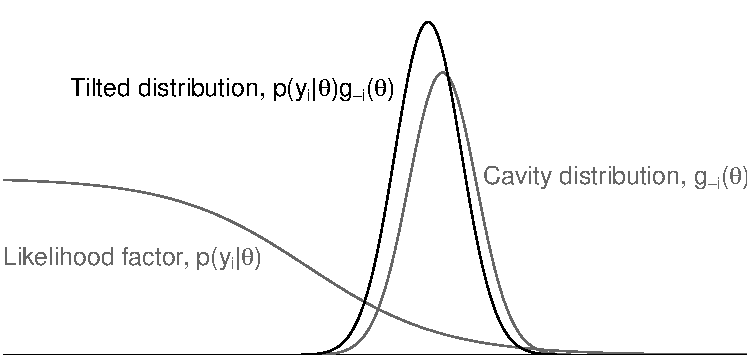
\includegraphics[width=.6\textwidth]{figures/separation.pdf}}
\caption{\em "Example of a step of an EP algorithm in a simple one-dimensional example, illustrating the stability of the computation even when part of the likelihood is far from Gaussian.  When performing inference on the likelihood factor $p(y_{(k)} | \phi)$, the algorithm uses the cavity distribution $g_{-k}(\phi)$ as a prior."}\label{fig:ep_tilted}
\end{figure}

% Tilted Distribution
With only site $k$'s approximating information removed, we then add back in the likelihood factor for site $k$ to create the \emph{tilted distribution},
\begin{align}
g_{\backslash k} (\phi) 
&\propto g_{-k}(\phi) p(y_{(k)} | x_{(k)}, \phi) 
&& \label{eq:ep_tilted}
\\\nonumber
&= g_{-k}(\phi) \int_{\alpha_{(k)}} p(y_{(k)} | x_{(k)}, \alpha_{(k)}, \phi) p(\alpha_{(k)} | \phi) d\alpha_{(k)}
\end{align}
which is equivalent to performing inference on the model $p(y_{(k)} | x_{(k)}, \alpha_{(k)}, \phi) p(\alpha_{(k)} | \phi)$ while using the cavity distribution $g_{-k}(\phi)$ as a prior, and then integrating out the local parameters $\alpha_{(k)}$ of the site. This interpretation of the tilted distribution is illustrated graphically in Figure \ref{fig:ep_tilted} \citep{Gelman+others:2017}, which demonstrates how using the cavity distribution $g_{-k}(\phi)$'s information from all of the other $K-1$ sites as a prior allows the titled distribution's inference to spend less time on areas of low posterior mass.

% Tilted Distribution Approximation
The algorithm then proceeds by first constructing a normal approximation $q_{\backslash k}(\phi)$ to the tilted distribution $g_{\backslash k}(\phi)$ by matching moments,
\begin{align}
g_{\backslash k} (\phi) 
\approx q_{\backslash k}(\phi) = N(\phi | r_{\backslash k}, Q_{\backslash k}). 
\label{eq:ep_tilted_approx}
\end{align}

The tilted distribution's normal approximation $q_{\backslash k}(\phi)$ then assists in creating the new site approximation by removing the information from the other $k' \neq k$ sites and prior,
\begin{align}
g_k^{new} 
&\approx \frac{q_{\backslash k}(\phi)}{g_{-k}(\phi)} 
= N(\phi | r_k^{new}, Q_k^{new}),
\end{align}
where the new site approximation's natural parameters are computed by
\begin{align}
Q_k^{new}
&= Q_{\backslash k} - Q_{-k}, \qquad
r_k^{new}
= r_{\backslash k} - r_{-k}. \label{eq:ep_site_approx}
\end{align}

% New Global Approximation
At the end of each iteration, after having conducted inference on all $k$ sites, the global approximation updates to
\begin{align}
g^{new}(\phi) 
&= p(\phi) \prod_k g_k^{new}(\phi) 
= N(\phi | r^{\rm new}, Q^{\rm new}),
\end{align}
where the natural parameters of the new global approximation are calculated as
\begin{align}
Q^{\rm new} 
&= Q_0 + \sum_{k} Q_k^{\rm new}, \qquad
r^{\rm new}
= r_0 + \sum_{k} r_k^{new}.
\end{align}
 
% Algorithm
Iterating the site updates in sequence or in parallel thus gives the following algorithm \citep{Gelman+others:2017}.
\\[2mm]
\begin{minipage}{\linewidth}
\begin{framed}
General expectation propagation algorithm
\begin{enumerate}
\item Choose initial site approximations $g_k(\phi)$.
\item Repeat for $k \in \{1,2,\dots,K\}$ (in serial or parallel batches) until all site approximations $g_k(\phi)$ converge:
    \begin{enumerate}
    \item Compute the cavity distribution, $g_{-k}(\phi) \propto g(\phi)/g_k(\phi)$.
    \item Compute the tilted distribution, $g_{\backslash k}(\phi) \propto g_{-k}(\phi) p(y_{(k)} | \phi) $
    \item \label{alg:tilted_approx} Update site approximation $g_k(\phi)$ so that $g_k(\phi) g_{-k}(\phi)$ approximates $g_{\backslash k}(\phi)$.
    \end{enumerate}
\end{enumerate}
\end{framed}
\end{minipage}\\[2mm]

% APPROXIMATING THE TILTED DISTRIBUTION
\subsection{Approximating the tilted distribution}
\label{subsec:ep_alg_approx}

In EP, if we use a multivariate normal family for the site approximations as described previously, the tilted distribution approximation in step~\ref{alg:tilted_approx} can be achieved by matching the first and second moments of $g_k(\phi)g_{-k}(\phi)$ to those of the possibly intractable tilted distribution $g_{\backslash k}(\phi)$. This corresponds to minimizing the Kullback-Leibler divergence $\operatorname{KL}(g_{\backslash k}(\phi) || q(\phi))$. For low dimension problems, this moment matching can be performed analytically \citep[e.g.][]{Opper+Winther:2000,Minka:2001b} or reasonably quickly using quadrature \citep[e.g.][]{Zoeter+Heskes:2005}. In higher dimensions, however, analytic solutions are generally nonexistent and quadrature error becomes intractable.

As such, for higher dimensions, feasible alternatives to approximating the titled distribution include matching the mode via Laplace methods, minimizing the reverse KL divergence via variational inference, and using numerical simulations via Monte Carlo \citep{Gelman+others:2017}. While Laplacian methods offer numerous computational advantages and variational inference offers guarantees about the global divergence minimization, we implement the simulation based approach in this paper as a proof of concept to demonstrate how beneficial distributed EP can be for the most demanding approximation algorithm.

Under the MCMC framework, simulations are used to sample from the tilted distribution at each step and set the moments of the approximating family. Specifically, this is accomplished by sampling from the joint tilted distribution in (\ref{eq:ep_tilted}) (i.e. without marginalizing the local parameters),
\begin{align}
g_{\backslash k} (\phi, \alpha_{(k)}) 
&= g_{-k}(\phi) p(y_{(k)}  | x_{(k)}, \alpha_{(k)}, \phi) p(\alpha_{(k)} | \phi),
\end{align}
which is equivalent to doing inference on the model $p(y_{(k)}  | x_{(k)}, a_{(k)}, \phi) p(a_{(k)} | \phi)$ while using $g_{-k}(\phi)$ as a prior. The MCMC samples from the joint distribution can then be approximated by a multivariate normal,
\begin{align}
g_{\backslash k} (\phi, {\bf a}_{(k)}) 
&\approx q(\phi, {\bf a}_{(k)}) = \normal(\phi, \alpha_{(k)} | r_{\backslash k}^* | Q_{\backslash k}^*),
\label{eq:ep_joint_tilted_approx}
\end{align}
at which point it is trivial to integrate out $\alpha_{(k)}$ and arrive at the marginal distribution $q_{\backslash k}(\phi)$ in (\ref{eq:ep_tilted_approx}).

The advantage of combining this approach with parallel EP is that the tilted approximation sampling only uses a fraction $1/K$ of the data (and parameters) per site. Since MCMC computations scale linearly in the number of data points, and superlinearly in the number of parameters, this is a huge computational advantage.

% KEEPING THE COVARIANCE POSITIVE DEFINITE
\subsection{Keeping the covariance matrix positive definite}
\label{subsec:ep_alg_eigens}

In Equation~ \ref{eq:ep_site_approx}, the last update step in each EP iteration, the approximated natural parameters $Q_{\setminus k}$ and $r_{\setminus k}$ of the tilted distribution are used together with the parameters $Q^{\rm new}_{- k}$ and $r^{\rm new}_{- k}$ of the cavity distribution to determine the new site approximation parameters $Q^{\rm new}_{k}$ and $r^{\rm new}_{k}$. Since the difference between the two positive definite matrices is not itself necessarily positive definite, there are situations in which the site approximation can be improper; this effectively breaks the EP algorithm.

The solution we propose for this problem is to smooth the tilted distribution's natural parameters with those of the cavity distribution. This can be achieved by taking a smoothing factor $\delta \in [0,1]$ and creating
\begin{align*}
Q^n_k = (1 - \delta^n) \cdot Q^{\rm old}_k + \delta^n \cdot Q^{\rm new}_k, \qquad
r^n_k = (1 - \delta^n) \cdot r^{\rm old}_k + \delta^n \cdot r^{\rm new}_k, \nonumber
\end{align*}
for $n \in \mathbb{N}$. One can then keep increasing $n$ until either $(Q^n_k)^{-1}$ is positive definite (in which case $Q^n_k$ and $r^n_k$ become the new approximation) or $\delta^n$ is smaller than some threshold $\epsilon$ (in which case we discard this site's update and keep the approximation the same as it was before). 